\section{Type checking}
XQuery/XPath has a well-defined type hierarchy.
\begin{figure}[h!]
  \centering
    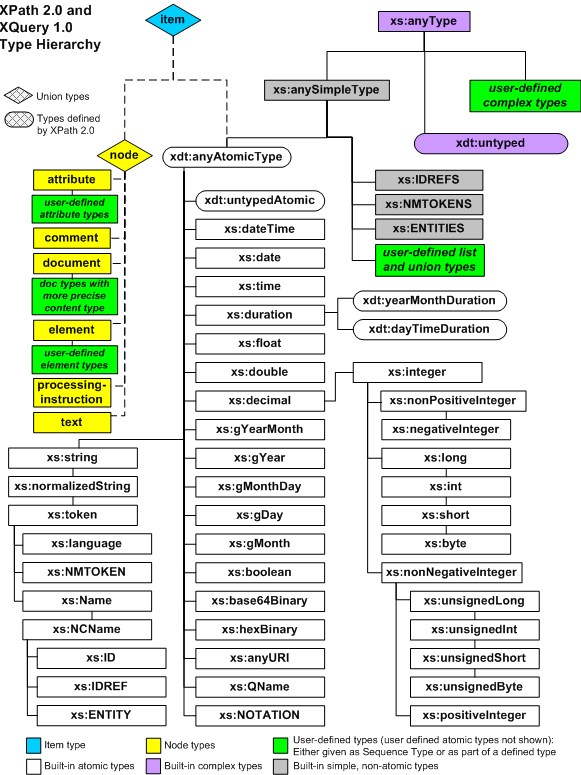
\includegraphics[scale=0.5]{img/xpathtypehierarchy}
  \caption{XQuery/XPath type hierarchy \cite{w3c04} (copyright
  \copyright W3C)}
\end{figure}
Here is a short overview of the basic type system:
\begin{itemize}
  \item Node types
    \begin{itemize}
      \item element()
      \item attribute()
      \item text()
      \item commment()
      \item document-node()
      \item processing-instruction()
    \end{itemize}
  \item Structure types
    \begin{itemize}
      \item Atomic types (xs:integer, xs:string, ..)
      \item Simple types (list, union)
      \item Complex types (user-defined types from an XML schema, except
      xs:anyType and xdt:untyped)
    \end{itemize}
\end{itemize}

Atomic types are strongly typed except xs:untypedAtomic, xs:anyURI, as well as
numerical types (xs:integer, xs:double, ..). Non-atomic simple types as well as
complex types are both strongly typed.

Proper type checking requires implementation of type inference and type
synthesis. This requires a stable abstract syntax tree and advanced data flow
analysis techniques to be feasible. Due to the inherent limitations in this
project, type checking has not been implemented - however the possibility of
this is discussed in section \ref{sect:summary:future_work}.

\underline{\textbf{\LARGE //TODO:}}
\begin{itemize}
  \item Dynamic vs. Static typing
  \item Strong vs. Weak (what and when)
  \item Type inference
  \item Michael Rys
\end{itemize}

\underline{\textbf{\LARGE //ODOT:}}